
\documentclass{article}

\usepackage{verbatim}
\usepackage{enumerate}
\usepackage{graphicx} % Required to insert images
\usepackage{fancyhdr} % Required for custom headers
\usepackage{extramarks} % Required for headers and footers
\usepackage{amsmath}
\usepackage{amssymb}
\usepackage{bbm}

% Margins
\topmargin=-0.45in
\evensidemargin=0in
\oddsidemargin=0in
\textwidth=6.5in
\textheight=9.0in
\headsep=0.25in 

\linespread{1.1} % Line spacing

% Set up the header and footer
\pagestyle{fancy}
\lhead{Linear Algebra with Application\\
to Engineering Computation}
\chead{}
\rhead{CME 200/ME300A\\
M. Gerritsen\\
Fall 2013}
\headheight = 40pt



%th in the exponent (e.g. when writing ith, instead use i$\eth$)
\newcommand{\tth}{^{\text{th}}}


%math symbols such as R
\newcommand{\I}{\ensuremath{\operatorname{I}}}
\newcommand{\One}[1]{\ensuremath{\mathbbm{1}_{\left \{ #1 \right \}}}}
\newcommand{\E}{\ensuremath{\mathbb{E}}}
\newcommand{\var}{\ensuremath{\operatorname{Var}}}
\newcommand{\cov}{\ensuremath{\operatorname{Cov}}}
\newcommand{\R}{\ensuremath{\mathbb{R}}}
\newcommand{\N}{\ensuremath{\mathbb{N}}}
\newcommand{\eqD}{\ensuremath{\overset{\mathcal{D}}{=}}}


%short-cuts for Greek letters
\newcommand{\al}{\alpha}
\newcommand{\dlt}{\delta}
\newcommand{\eps}{\epsilon}
\newcommand{\la}{\lambda}

%times (cross-product)
\newcommand{\x}{\times}
%inverse
\newcommand{\inv}{^{-1}}
%cond
\newcommand{\cond}{\mathrm{cond}}
%trace
\newcommand{\trace}{\mathrm{trace}}
\newcommand{\tr}{\mathrm{tr}}

\newcommand{\twith}{\text{ with }}
\newcommand{\tand}{\text{ and }}
\newcommand{\tfor}{\text{ for }}
\newcommand{\tor}{\text{ or }}
\newcommand{\tat}{\text{ at }}

\newcommand{\ip}{_{i+1}}
\newcommand{\im}{_{i-1}}

\newcommand{\half}{\frac{1}{2}}
\newcommand{\oneby}[1]{\frac{1}{#1}}
\newcommand{\overto}[1]{\overset{#1}{\longrightarrow}} 
 
\renewcommand\headrulewidth{0.4pt} % Size of the header rule
\renewcommand\footrulewidth{0.4pt} % Size of the footer rule

\setlength\parindent{0pt} % Removes all indentation from paragraphs

%----------------------------------------------------------------------------------------
%	DOCUMENT STRUCTURE COMMANDS
%	Skip this unless you know what you're doing
%----------------------------------------------------------------------------------------

% Header and footer for when a page split occurs within a problem environment
\newcommand{\enterProblemHeader}[1]{
\nobreak\extramarks{#1}{#1 continued on next page\ldots}\nobreak
\nobreak\extramarks{#1 (continued)}{#1 continued on next page\ldots}\nobreak
}

% Header and footer for when a page split occurs between problem environments
\newcommand{\exitProblemHeader}[1]{
\nobreak\extramarks{#1 (continued)}{#1 continued on next page\ldots}\nobreak
\nobreak\extramarks{#1}{}\nobreak
}

\setcounter{secnumdepth}{0} % Removes default section numbers
\newcounter{homeworkProblemCounter} % Creates a counter to keep track of the number of problems

\newcommand{\homeworkProblemName}{}
\newenvironment{homeworkProblem}[1][Problem \arabic{homeworkProblemCounter}]{ % Makes a new environment called homeworkProblem which takes 1 argument (custom name) but the default is "Problem #"
\stepcounter{homeworkProblemCounter} % Increase counter for number of problems
\renewcommand{\homeworkProblemName}{#1} % Assign \homeworkProblemName the name of the problem
\section{\homeworkProblemName} % Make a section in the document with the custom problem count
\enterProblemHeader{\homeworkProblemName} % Header and footer within the environment
}{
\exitProblemHeader{\homeworkProblemName} % Header and footer after the environment
}
\newcommand\overmat[2]{%
  \makebox[0pt][l]{$\smash{\overbrace{\phantom{%
    \begin{matrix}#2\end{matrix}}}^{\text{$#1$}}}$}#2}

\newcommand{\problemAnswer}[1]{ % Defines the problem answer command with the content as the only argument
\noindent\framebox[\columnwidth][c]{\begin{minipage}{0.98\columnwidth}#1\end{minipage}} % Makes the box around the problem answer and puts the content inside
}

\title{Assignment 8}
\date{Issued: November 20, 2013}
\author{Due: December 4, in class\\
No late assignments accepted}

%----------------------------------------------------------------------------------------

\begin{document}
\maketitle
\thispagestyle{fancy}
\textbf{Important:}
\begin{itemize}
\item Give complete answers: Do not only give mathematical formulae, but explain what you are doing. Conversely, do not leave out critical intermediate steps in mathematical derivations.
\item Write your \textbf{name} as well as your \textbf{Sunet ID} on your assignment. \textbf{Please staple pages together.}
\item Questions preceded by  $\star$  are harder and/or more involved.
\item \textbf{Include code with your assignment}
\item Comment any graphs and plots on the same page as the graph or plot itself.
\end{itemize}


% Problem 1
\begin{homeworkProblem}
Consider the symmetric matrix
\[ A = \begin{bmatrix} 9 & -7 \\ -7 & 17 \end{bmatrix} \]
\begin{enumerate}[(a)]
\item Compute the eigenvalues and eigenvectors of $A$. Do this by hand.
\item Show that the eigenvectors of $A$ are orthogonal.
\end{enumerate}
\end{homeworkProblem}


% Problem 2
\begin{homeworkProblem} 
True or False? If true, prove the statement. If false, you need only provide a counterexample.
\begin{enumerate}[(a)]
\item If the $n \x n$ matrix $B$ is formed from the $n \x n$ matrix $A$ by swapping two rows of $A$, then $B$ and $A$ have the same eigenvalues.
\item Any invertible $n \x n$ matrix $A$ can be diagonalized.
\item A singular matrix must have repeated eigenvalues.
\item If the $n \x n$ matrices $A$ and $B$ are diagonalizable, so is the matrix $AB$.
\item Let $A$ be an $n \x n$ matrix. 
      \begin{enumerate}[(i)]
        \item The eigenvalues of $A$ and $A^T$ are the same.
        \item The eigenvalues and eigenvectors of $A^TA$ and $AA^T$ are the same.
      \end{enumerate}
\end{enumerate}
\end{homeworkProblem}


% Problem 3
\begin{homeworkProblem}
A rabbit population $r$ and a wolf population $w$ are related according to the following system of differential equations:
\begin{eqnarray*}
\frac{dr}{dt} &=& 5r - 2w \\
\frac{dw}{dt} &=& r + 2w
\end{eqnarray*}
Here $t$ denotes time.
\begin{enumerate}[(a)]
\item If initially (at $t = 0$) there were 100 rabbits and 50 wolves, find the numbers of rabbits and wolves as a function of time $t$.
\item Design a matrix $A$ for the above system such that the populations coverge to a finite non-zero limit as $t$ goes to infinity.
\end{enumerate}
\end{homeworkProblem}

% Problem 4
\begin{homeworkProblem}
Heat Equation. We look at the matrix
\[A = \begin{bmatrix} -2 & 1 & 0 \\ 1 & -2 & 1 \\ 0 & 1 & -2 \end{bmatrix} \]
\begin{enumerate}[(a)]

% Problem 4 (a)
\item Find the eigenvalues of $A$ and the corresponding eigenvectors. $A$ is symmetric, so the eigenvectors should be orthogonal. Check that this is the case. 

% Problem 4 (b)
\item Give the algorithm of the power method that can be used to find the largest eigenvalue (in absolute value) of $A$. 

% Problem 4 (c)
\item Execute this algorithm, either by hand or with matlab. As initial vector take one of the unit vectors, produce a figure showing the computed approximations as a function of iteration step. Repeat with an initial vector equal to an eigenvector corresponding to either of the two smallest eigenvalues. Observe that the algorithm still converges. but slower than before (round-off error accumulation helps in this case as we discussed in class). \\ \\
Note: The matrix is well-conditioned and the round-off error will not accumulate particularly fast. Make sure you force the iteration to run for a while (we have found at least 60 iterations works) because you are only testing the relative error in successive iterates of the eigenvalues.

% Problem 4 (d)
\item Instead of looking at this $3 \x 3$ matrix, take $10 \x 10$ (or larger if you like) matrix with the same tridiagonal structure ($-2$ on the main diagonal and $1$ on the subdiagonals). Find all eigenvalues of this larger matrix using the $QR$ iterations. Check your answers against the eigenvalues computed by matlab using the \texttt{eig} command. Again, motivate your convergence criterion. 

% Problem 4 (f)
\item Since the heat equation discretization was an example of numerically solving a differential equation, the plotting of solutions was rather important. Since we just computed eigenvectors, we might be interested to see what the eigenvectors look like when plotted. Consider $102 \x 102$ discretization for the heat equation so that the matrix $A$ is $100 \x 100$. Use the \texttt{eig} command in matlab to obtain the eigenvectors $\vec{v}^{(1)}, \ldots, \vec{v}^{(100)}$ for $-A$ (this is $-A$ so there are positive 2s on the diagonal). For $j = 1, \ldots, 5$, plot $\sqrt{101}\vec{v}^{(j)}$ as we have done in previous homeworks (remember the boundary values). \\ \\
Now verify for yourself that the functions $u_j(t) = \sqrt{2}\sin (j\pi t)$ for $j = 1, 2, 3, \ldots$ satisfy the differential equation, 
\[ -\frac{d^2u_j}{dt^2} = \lambda u_j, \ \ \lambda = (j \pi)^2, \ \ u_j(0) = u_j(1) = 0, \ \ \int_0^1 u_j(t)^2 dt = 1.\]
How do the eigenvectors $\vec{v}^{(j)}$ of $-A$ compare to the ``eigenfunctions'' $u_j(t)$ of the differential equation? What significance does the factor $\sqrt{101}$ have when plotting $\sqrt{101}\vec{v}^{(j)}$ (think about a Riemann sum approximation of the above integral)?
\end{enumerate}
\end{homeworkProblem}
  
% Problem 5
\begin{homeworkProblem}
In this problem we consider a small mass-spring system, consisting of 2 masses that are connected to each other and to fixed walls by three identical springs as shown in the figure. 

\begin{figure}[!h]
\centering
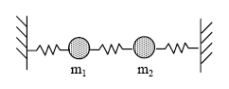
\includegraphics[width=2in]{mass_spring.png}
\caption{Mass-Spring System.}
\end{figure}

At time $t = 0$, we gtive the first mass $m_1$ a small displacement. As a result the mass-spring system will start to move in an oscillatory fashion. If the masses are both equal to 1, the system of equation that describes the displacement of the masses is given by 
\[ \frac{d^2\vec{u}}{dt^2} = A\vec{u}, \]
where
\[ \vec{u} = \begin{bmatrix} u_1 \\ u_2 \end{bmatrix}, \]
with $u_1 \tand u_2$ are the displacements of $m_1 \tand m_2$, respectively, and 
\[ A = \begin{bmatrix} -2 & 1 \\ 1 & -2 \end{bmatrix}. \]
We take the initial conditions (we need two of them for a second order differential equation) to be 
\[ \vec{u}(0) = \begin{bmatrix} 1 \\ 0 \end{bmatrix}, \ \ \frac{d\vec{u}}{dt}(0) = \begin{bmatrix} 0 \\ 0 \end{bmatrix}, \]

\begin{enumerate}[(a)]

% Problem 5 (a)
\item Find the matrices $Y$ and $\Lambda$ such that $A = Y \Lambda Y^{-1}$, with $Y$ orthogonal, and $\Lambda$ diagonal.

% Problem 5 (b)
\item Using this decomposition of $A$, show that we can transform the system of differential equations to
\[ \frac{d^2\vec{z}}{dt^2} = \Lambda \vec{z}, \ \ \vec{z} = Y^T \vec{u}.\]
The system for $\vec{z}$ is now ``decoupled'' so you can solve each component individually since they do not depend on each other. Solve the system of equations for $\vec{z}$ and from it find the displacements $u_1$ as a function of time $t$.

% Problem 5 (c)
\item If the masses are not equal, the system of differential equations describing the motion of the mass-spring system is instead given by 
\begin{equation} \label{mass-spring} M\frac{d^2\vec{u}}{dt^2} = A\vec{u}, \ \ M = \begin{bmatrix} m_1 & 0 \\ 0 & m_2 \end{bmatrix}.\end{equation}
We guess solution will be of the form $\vec{u}(t) = e^{i \omega t} \vec{v}$, where $\omega \tand \vec{v}$ are quantities determined by $M \tand A$. Plug in $\vec{u}(t) = e^{i \omega t} \vec{v}$ and show that finding $\omega \tand \vec{v}$ corresponds to the so-called ``generalized eigenvalue problem''
\[ A\vec{v} = \lambda M \vec{v},\]
with $\lambda = (i \omega)^2$. \\ \\
Now set $m_1 = 1$ and $m_2 = 2$. The characteristic polynomial for the generalized eigenvalue problem is given by $\det(A - \lambda M) = 0$. Solve the characteristic polynomial to find the two generalized eigenvalues $\lambda_1, \lambda_2$ (or if you wish, the two values of $\omega$ since $\lambda = (i \omega)^2$) and the two generalized eigenvectors $\vec{v}_1, \vec{v}_2$. Then give the solution to the differential equation in (\ref{mass-spring}).
\end{enumerate}
\end{homeworkProblem}
\end{document}
 
 
 
